\documentclass{beamer}

%\setbeameroption{show notes}

% Vary the color applet  (try out your own if you like)
%\colorlet{structure}{red!65!black}

%\beamertemplateshadingbackground{yellow!100}{white}

%\usepackage{beamerthemesplit}
\usepackage{tikz}
\usepackage{graphics}
\usepackage{graphicx}
\usepackage{hyperref}
\usepackage{setspace}
\usepackage{colortbl}
\usepackage{listings}
\usepackage{amsfonts}
\usepackage{amsmath}
\usepackage{multicol}

%\usetikzlibrary{shapes}

\newcounter{exercise}
\setcounter{exercise}{0}

\newenvironment{exercise}[1]
  {\stepcounter{exercise}\begin{block}{\bf Exercise \arabic{exercise}: #1}}
  {\end{block}}

\lstset{ %
language=Python,                % choose the language of the code
basicstyle=\footnotesize \tt,       % the size of the fonts that are used for the code
%numbers=left,                   % where to put the line-numbers
%numberstyle=\footnotesize,      % the size of the fonts that are used for the line-numbers
%stepnumber=2,                   % the step between two line-numbers. If it's 1 each line will be numbered
%numbersep=5pt,                  % how far the line-numbers are from the code
%backgroundcolor=\color{white},  % choose the background color. You must add \usepackage{color}
%showspaces=false,               % show spaces adding particular underscores
%showstringspaces=false,         % underline spaces within strings
%showtabs=false,                 % show tabs within strings adding particular underscores
%frame=single,                   % adds a frame around the code
%tabsize=2,                      % sets default tabsize to 2 spaces
%captionpos=b,                   % sets the caption-position to bottom
%breaklines=true,                % sets automatic line breaking
%breakatwhitespace=false,        % sets if automatic breaks should only happen at whitespace
%escapeinside={\%*}{*)}          % if you want to add a comment within your code
}

\usetheme{Madrid} 
\useinnertheme{rounded}
\usecolortheme{crane}

\definecolor{dredcolor}{rgb}{.5,0.0,0.0}
\definecolor{blackcolor}{rgb}{0.0,0.0,0.0}
\definecolor{dgreencolor}{rgb}{0.0,0.4,0.0}
\definecolor{dbluecolor}{rgb}{.02,.02,.808}
\newcommand{\dblue}{\color{dbluecolor}\bf}
\newcommand{\dgreen}{\color{dgreencolor}\bf}


\title[Cython]{Cython Tutorial}
\author[Seljebotn]{Dag Sverre Seljebotn \\ \texttt{d.s.seljebotn@astro.uio.no}}
\date{PyData 2012}
\institute{University of Oslo}

%\pgfdeclaremask{fsu}{fsu_logo_ybkgrd}
%\pgfdeclareimage[mask=fsu,width=1cm]{fsu-logo}{fsu_logo_ybkgrd}

%\logo{\vbox{\vskip0.1cm\hbox{\pgfuseimage{fsu-logo}}}}

\begin{document}

  \frame
  {
    \titlepage
    \begin{center}
    
\includegraphics[scale=0.4]{cython-logo.png}
    \end{center}
  }

\section[Introduction]{Introduction}
\frame{
  \frametitle{Getting set up}

{Tutorial source files should be on USB stick. Also:}
{\Large \texttt{http://github.com/dagss/cython-pydata12}}

~

Cython relies on:

\begin{itemize}
\item A C/C++ compiler (can be a problem on Windows)
\item Python development headers\\  (Ubuntu: \texttt{sudo apt-get install python-dev})
\end{itemize}
Using scientific Python distributions (such as EPD) solve both
of these.

~

\uncover<2->{If you distribute software in source code form, your users will
  need the above too.}

}


\frame{
  \frametitle{Cython at a glance}
  \begin{itemize}
    \item<+-> Cython is used for compiling Python-like code to machine-code
      \begin{itemize}
      \item superset of Python
      \item conditions and loops run 2-8x faster, overall
	30\% faster for plain Python code (vs. Py2.5, using PyBench)
      \end{itemize}
    \item<+-> In addition:
      \begin{itemize}
      \item Add types for speedups (hundreds of times)
      \item Easily use native libraries (C/C++/Fortran) directly
      \end{itemize}
    \item<+-> How it works:
	Cython code is turned into C code which uses the CPython API and runtime.
	\begin{itemize}
	\item Generated C code can be built and run without Cython installed
      \end{itemize}
    \item<+-> Has its share of warts, but works now!
  \end{itemize}

~

\uncover<4->{\bf Coding in Cython is like coding
in Python and C at the same time!}
}



\frame{
  \frametitle{Usecase 1: Library wrapping}

  \begin{itemize}
    \item Cython is a popular choice for writing Python interface
      modules for C libraries
    \item Works very well for writing a higher-level Pythonized wrapper
    \item For 1:1 wrapping other tools might be better suited,
depending on the exact usecase
  \end{itemize}

~

Examples: mpi4py, pyzmq, petsc4py, ...

}


\frame{
  \frametitle{Usecase 2: Performance-critical code}
  \begin{columns}[t]
    \begin{column}{0.3\textwidth}
      Python \\ High-level \\ Slow \\ No variables typed
    \end{column}
    \begin{column}{0.4\textwidth}
      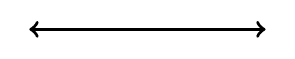
\begin{tikzpicture}
	\draw[<->, very thick]  (0, 0)  -- (3, 0);
      \end{tikzpicture}
    \end{column}
    \begin{column}{0.3\textwidth}
      C/C++/Fortran \\ Lower-level \\ Fast \\ All variables typed
    \end{column}
  \end{columns}
  

~

  \begin{itemize}
    \item<+-> Common procedure: Where speed is needed, use a compiled language, then wrap the
      code for use from Python
    \item<+-> Cython: Incremental optimization workflow
      \begin{itemize}
      \item Optimize, don't re-write
      \item Only the pieces you need
    \end{itemize}


~

Examples: scikits-image, pandas, Sage, ...

  \end{itemize}

}

% \Frame{

%   \tikzstyle{lib}=[rectangle,
%                    thick,
%                    minimum height=2cm,
%                    minimum width=1.5cm,
%                    draw=purple!80,
%                    fill=purple!20,
%                    font=\tiny]

%   \tikzstyle{clib}=[rectangle,
%                    thick,
%                    minimum height=1.5cm,
%                    minimum width=1.5cm,
%                    draw=blue!80,
%                    fill=blue!20,
%                    font=\tiny]

% \begin{tikzpicture}

%    \draw[very thick] (0,0) -- (10, 0);
%    \node[lib,anchor=north] (numpy) at (1, .5) {NumPy/SciPy};
%    \node[lib,anchor=north] (pytables) at (3, .5) {PyTables};
%    \node[lib,anchor=north] at (5, .5) {$\cdots$};

%    \node[clib] at (1, -3) (lapack) {LAPACK/BLAS};
%    \node[clib] at (3, -3) (hdf) {hdf5};

%    \draw[thick,->] (numpy.south) -- (lapack.north);
%    \draw[thick,->] (pytables.south) -- (hdf.north);

%    \node[circle, draw=yellow!80, fill=yellow!20, 
%          minimum width=2cm, minimum height=1cm, font=\tiny\bf] at (7, 0) {Cython code};

% \end{tikzpicture}
% }

\frame{
  \frametitle{Not a usecase: Static type checking}
  \begin{itemize}
    \item Cython is (partially) statically typed because it has too,
      not because it wants to
    \item You still need to run the program to catch a typo
  \end{itemize}
}


\frame{
  \frametitle{How Cython works}
  Cython code must be compiled. This happens in two stages:

~

  \begin{enumerate}
  \item<+-> A {\tt .pyx} file is compiled by Cython to a {\tt .c} file, containing
    the code of a Python extension module
  \item<+-> The {\tt .c} file is compiled by a C compiler
    \begin{itemize}
      \item Special compiler flags dictated by the Python installation must be used
    \end{itemize}
  \end{enumerate}

~

  \uncover<2->{
    The result is a {\tt .so} file (or {\tt .pyd} on Windows) which can be {\tt import}-ed
    directly into a Python session.
  }

~

\uncover<2->{If you are wrapping a C++ library, one can use C++ instead of C.}
}

\frame{
  \frametitle{Ways to build Cython code...}

  \begin{itemize}
  \item<+-> \texttt{distutils}: \texttt{setup.py}
  \item<+-> Simple cases: \texttt{pyximport} automatically compiles on Python import
  \item<+-> Advanced cases: Use a {\em real} build tool
    \begin{itemize}
    \item CMake, waf, SCons, Unix Makefiles, IDE projects...
    \end{itemize}
  \end{itemize}

}

\frame[containsverbatim]{
  \begin{exercise}{Building a Cython module}
\begin{enumerate}
 \item Write some Python code in {\tt example.pyx}
 \item Get {\tt https://github.com/dagss/cython-pydata12/hello}

\item To build: {\tt python setup.py build\_ext -i}
\begin{itemize}
\item {\tt python setup.py install} installs
\end{itemize}
\item Then simply {\tt import example}
\item Finally have a look at the generated C code
\end{enumerate}
\end{exercise}

}


\frame{
  \frametitle{The problem of getting benchmarks}
\begin{itemize}
\item<+-> CPU frequency scaling
\item<+-> Turbo-mode when running with one or two cores
\item<+-> Interruptions by operating system
\item<+-> Warm-start vs. cold-start
\item<+-> What numbers to quote: CPU-time or wall-time?
\end{itemize}
\uncover<+->{Remedies:}
\begin{itemize}
\item<+-> Disable turbo-mode (BIOS), disable CPU frequency scaling
\item<+-> Outer loop: Repeat benchmark many times, take {\em minimum}
  \begin{itemize}
  \item Purpose: Avoid OS interruptions, get a warm-start, help against
    frequency scaling
  \end{itemize}
\item<+-> Inner loop: Repeat benchmark many times, {\em take average of wall time}
  \begin{itemize}
  \item Purpose: Get better timer resolution
  \end{itemize}
\item<+-> Make sure the Cython-part of the benchmark does enough work,
  or you'll be benchmarking the (slow) speed of a Python for-loop
\end{itemize}
}


\defverbatim[colored]\testcode{%
\lstset{emph={cdef, int, float},emphstyle=\color{blue}} 
\begin{lstlisting}
cdef int two = 2
def func(int x):
    cdef int i, y = two * x
    cdef float z
    z = x / 3
    print z**2
    return z
\end{lstlisting}}

\frame{
  \frametitle{Faster code: Adding types}

\uncover<+->{
Variables can be typed with a C-like notation:
\testcode
}

\begin{itemize}
\item<+-> {\bf Types are optional,} and even slightly discouraged. Always check that you have a good reason for using them.
\item<+-> All C types are available
\item<+-> Conversion to and from Python objects happen automatically.
\item<+-> Note that Python {\tt float} and {\tt int} and C {\tt float} and {\tt int}
are different things.
\end{itemize}
}

\frame[containsverbatim]{
  \frametitle{Faster code: cdef functions}
  Python function calls can be expensive -- in Cython doubly so because
  one might need to convert to and from Python objects to do the call.

~

Therefore Cython provides a syntax for declaring a Cython-only function:
\lstset{emph={cdef, cpdef, double},emphstyle=\color{blue}} 
\begin{lstlisting}
cdef double f(double x): return x**3 + 2*x**2
\end{lstlisting}

~

The downside is that the function is not available from Python-space.
Using {\tt cpdef} makes a fast version available to Cython and a slower one
to Python:
\begin{lstlisting}
cpdef double f(double x): return x**3 + 2*x**2
\end{lstlisting}

}


\frame[containsverbatim]{

\begin{exercise}{Adding types}
Add types etc. to speed up the following code (name the file
{\tt integrate.pyx} for future reference):
\begin{lstlisting}
from __future__ import division
def f(x): return 1/(x**3 + 2*x**2)
def integrate_f(a, b, N):
    s = 0
    dx = (b-a)/N
    for i in range(N):
        s += f(a+i*dx)
    return s * dx
\end{lstlisting}
\begin{itemize}
\item Use the {\tt double} type for function values and domain, and
{\tt ssize\_t} for integers.

\item Expect about 100x speedup. It is easy to miss typing a variable;
experiment and see what happens to speed then.

\item Use the \verb@-a@ switch to the \verb@cython@ command-line tool;
the generated view of the code explains the speed differences

\item Experiment with letting \verb@f@ be declared \verb@cdef@ vs. \verb@cpdef@.
\end{itemize}
\end{exercise}
}


\frame[containsverbatim]{ \frametitle{Raising exceptions from {\tt cdef} functions}
For speed reasons, some manual exception declarations must be done
on {\tt cdef} functions capable of raising exceptions.

~

You can always add "{\tt except *}" and not worry about this though.
\begin{block}{}
\begin{lstlisting}
cdef int is_monday() except -2:
    # Must never return -2 explicitly!
    return time.localtime().tm_wday == 0

cdef int divide(int a, int b) except? 45345:
    # If result is 45345, make an additional check
    return a // b # possible ZeroDivisionError

cdef int divide(int a, int b) except *:
    # I'd rather not bother, just ask Python
    return a // b
\end{lstlisting}
\end{block}
}


\section{Calling C functions}

\frame[containsverbatim]{
  \frametitle{Calling C functions}
One {\em can} do ``{\tt from math import sin}'' to get
Python's {\tt sin} function. Calling C's {\tt sin} function
is faster though:
\begin{lstlisting}
cdef extern from "math.h":
    double sin(double)
# or:
# from libc.math cimport sin

cdef double f(double x):
    return sin(x * x)
\end{lstlisting}

Note that one must ``redeclare'' the function from {\tt math.h}
for the benefit of Cython. In the C compilation stage, only
the declaration in {\tt math.h} is seen.
}

\frame[containsverbatim]{
  \frametitle{Calling C functions}
When calling C functions, one must take care to link in the appropriate
libraries. In {\tt setup.py}:

\lstset{emph={libraries},emphstyle=\color{blue}} 
\begin{lstlisting}
...
    Extension("integrate", ["integrate.pyx"],
              libraries=["m"]) # Unix-like specific
...
\end{lstlisting}
}

\frame[containsverbatim]{

\begin{exercise}{Call a C function}
Just make sure you now know how to calculate $\int_a^b \textrm{sin}(x^2) \; \textrm{d}x$.

Check the speed difference between calling Python's \texttt{sin} and C's \texttt{sin}.

\end{exercise}


}

\section{NumPy and Cython}

\frame{ \frametitle{NumPy and Cython}

\uncover<+->{
  \begin{itemize}
  \item Cython provides fast access to NumPy arrays
    \begin{itemize}
    \item As long as datatype and dimensionality of all arrays is known at compile-time!
    \end{itemize}
  \item 1000x speedup over pure Python loops in extreme cases
  \end{itemize}
}

~

\uncover<+->{
Some usecases:

\begin{itemize}
\item Make manual for-loop-style programming feasible
\item<+-> Optimize an array expression like \texttt{1.2 * a + b + np.sqrt(c)}
  \begin{itemize}
  \item Helps because it reduces memory bandwidth
  \item \texttt{numexpr} and \texttt{Theano} solves the same problem
  \end{itemize}
\item<+-> Push data between NumPy arrays and C/C++/Fortran libraries
\end{itemize}
}

}

\frame[containsverbatim]{

\begin{exercise}{Optimize pixel-domain convolution}
Check out the \texttt{integrate} example and speed it up.

\begin{itemize}
 \item Use the \texttt{float} type (32-bit floating point data) for values,
   \texttt{ssize\_t} for indices
 \item NumPy arrays should be typed:
\begin{verbatim}
import numpy as np
cimport numpy as cnp
cnp.import_array()
def convolve2d(cnp.ndarray[float, ndim=2] f, ...)
\end{verbatim}

  \item Headers needed for the C compiler as well.
    In \texttt{setup.py}:
\begin{verbatim}
Extension("cy_convolve", ["cy_convolve.pyx"],
          include_dirs=[np.get_include()])
\end{verbatim}
\end{itemize}
\end{exercise}

}


\frame[containsverbatim]{
  \frametitle{Object-oriented programming}
  Cython has two kinds of classes:
  \begin{itemize}
    \item Normal Python classes. These are exactly like Python's classes.
    \item Extension types/``cdef classes''
      \begin{itemize}
	\item Store typed attributes (avoid converting to/from Python object)
	\item Faster method calls when called from Cython
        \item Between different Cython modules, \texttt{.pxd}-files are needed
          to export the cdef class interface
      \end{itemize}
  \end{itemize}
\begin{lstlisting}
cdef class MyClass:
    cdef int value
    cpdef int some_method(self, int arg):
        ...
\end{lstlisting}

~

Normal Python classes (also in pure Python code)
can inherit from cdef classes, but not the other way around.
}

\frame[containsverbatim]{
  \frametitle{cdef class polymorphism}
  Methods of cdef class objects can be called much faster than methods 
  on regular objects, {\em if} the variable is typed.

~

\begin{lstlisting}
untyped = MyClass(arg1, arg2)
cdef MyClass typed = untyped
untyped.some_cpdef_method() # slow
typed.some_cpdef_method() # fast
\end{lstlisting}
  
~
  Regular Python classes can not be used as the type of
  a variable.
}

\frame[containsverbatim]{
  \frametitle{cdef class attributes}
  Attributes are different from regular classes:
  \begin{itemize}
    \item All attributes must be pre-declared at compile-time
    \item Attributes are by default only accessible from Cython (typed access)
    \item Properties can be declared to make the attribute accessible from Python-space
  \end{itemize}

~

\begin{lstlisting}
cdef class SineWave(DoubleFunction):
    cdef double offset # not available in Python-space
    cdef public double frequency # available in Python-space
    property period:
        def __get__(self): return 1.0 / self.frequency
	def __set__(self, value): self.frequency = 1.0 / value
    ...
\end{lstlisting}

}

\frame{
  \frametitle{cdef class caveats}
  Special methods have some differences from regular classes:
  \begin{itemize}
    \item<+-> {\tt \_\_cinit\_\_} is, unlike {\tt \_\_init\_\_}, guaranteed to be
    called exactly once per object
    \begin{itemize}
      \item {\tt \_\_init\_\_} is available as well
      \item Take care: Might be called before the Python object has
	been fully constructed!
      \item Rationale: Improper initialization of C attributes can cause leaks or crashes.
    \end{itemize}
    \item<+-> {\tt \_\_dealloc\_\_} is called when the object is deallocated
    \item<+-> Arithmetic operators, pickling etc. are different as well
  \end{itemize}
}

\frame[containsverbatim]{
  \frametitle{The None issue}
  \begin{itemize}
    \item For convenience, variables declared as having a cdef class type can
      be assigned {\tt None}.
    \item By default, accessing None in such a ``typed'' fashion will
      lead to undefined behaviour (hopefully a crash). Always test with {\tt is None}
      first!
    \item The {\tt nonecheck} {\em compiler directive} will raise an exception instead;
      but slows down all such accesses.
  \end{itemize}

\begin{lstlisting}
import cython
@cython.nonecheck(True)
def func():
    cdef MyClass obj = None
    try:
        print obj.myfunc() # raises exception
    except AttributeError:
        pass
    with cython.nonecheck(False):
        print obj.myfunc() # hope for a crash!
\end{lstlisting}

}

\frame[containsverbatim]{

  \begin{exercise}{Using cdef classes in the integration example}
    Until now, the function to integrate has been hardcoded.
    Let's use cdef classes to create callbacks without too much of a penalty.

\end{exercise}
}


% \begin{frame}[containsverbatim]
%   \frametitle{What does Cython look like in the future? (we hope...)}

%   \begin{itemize}
%   \item Fused types:
% \begin{verbatim}
% def compute_foo(np.ndarray[floating_t] a): ...
% \end{verbatim}
%   \end{itemize}
% \end{frame}

% \begin{frame}[containsverbatim]
%   \frametitle{What does Cython look like in the future? (we hope...)}

%   \begin{itemize}
%   \item Fused types:
% \begin{verbatim}
% def compute_foo(np.ndarray[floating_t] a): ...
% \end{verbatim}
%   \item Typed memoryviews.
%     \begin{itemize}
%     \item Rather than {\em optimize memory access}, we 
%     \end{itemize}
% \begin{verbatim}
% def compute_foo(double[:] a, double[:] b):
%     cdef double[:] c = a * a + b
%     ...
% \end{verbatim}
%   \end{itemize}
% \end{frame}

\end{document}
